\chapter{Design}
\label{sec:design}

% Ist das zentrale Kapitel der Arbeit. Hier werden das Ziel sowie die
% eigenen Ideen, Wertungen, Entwurfsentscheidungen vorgebracht. Es kann
% sich lohnen, verschiedene Möglichkeiten durchzuspielen und dann
% explizit zu begründen, warum man sich für eine bestimmte entschieden
% hat. Dieses Kapitel sollte - zumindest in Stichworten - schon bei den
% ersten Festlegungen eines Entwurfs skizziert werden.
% Es wird sich aber in einer normal verlaufenden
% Arbeit dauernd etwas daran ändern. Das Kapitel darf nicht zu
% detailliert werden, sonst langweilt sich der Leser. Es ist sehr
% wichtig, das richtige Abstraktionsniveau zu finden. Beim Verfassen
% sollte man auf die Wiederverwendbarkeit des Textes achten.

% Plant man eine Veröffentlichung aus der Arbeit zu machen, können von
% diesem Kapitel Teile genommen werden. Das Kapitel wird in der Regel
% wohl mindestens 8 Seiten haben, mehr als 20 können ein Hinweis darauf
% sein, daß das Abstraktionsniveau verfehlt wurde.

% Die Lösung kurz vorstellen. also du hast dich für die lösung mit dem dc network entschieden und das wurde bisher noch nicht vorgeschlagen in der wissenschaft. Dann sagen bevor du das prinzip vorstellt werden erstmal alle Teilnehmer, die in dem System vorkommen, vorgestellt. dazu auch das bild aus der technischen richtlinie benutzen, wo smartmeter und smart meter admin. welche netzwerke also han etc...
%Dann sagen, dass du erstmal auf das angreifermodell eingehst und dann dc netz erklären und dann die lösung vorschlagen.
%die lösung wurde noch nicht diskutiert, weil in der wissenschaft immer davon ausgegangen wurde, dass smart meter nicht sicher sind,wir gehen davon aus, dass ein smart meter vertraut werden kann und das man deshalb auch nicht auf das billing eingehen muss, weil das smart meter korrekt arbeitet und das billing deshalb trivial ist. der stromanbieter kann auch prüfen  bzw. die logeinträge sind fälschungssicher.

This chapter outlines the conceptual solution of this thesis to achieve privacy-preserving smart meters. The proposed protocol can be categorized as aggregation without a trusted third party. Before discussing the conceptual solution, the technical guideline from the BSI will be explained. The BSI is the cyber-security authority of the German government and is responsible for critical infrastructures such as smart grids in Germany.  The technical guideline TR-03109 resolves all security standards and security concepts that must be met by all power grid providers in Germany. Therefore, the technical guideline gives a good overview of the actual structure of the German power grid. After getting an overview of the power grid and its participants, an attacker model will be designed. The attacker model will introduce all necessary participants, what their motives are and what malicious motives they might pursue. Finally, the security protocol will be presented. It will be shown how the protocol can be integrated into the technical policy and how different potentially malicious participants are handled.

\section{Technical guideline TR-03109}
This paragraph will discuss the technical guideline published by the BSI (Federal Office for Information Security). The BSI is the entity of the German federal government that deals with digital security issues and issues recommendations as well as mandatory security guidelines for critical infrastructures. Among other things, technical guidelines are published in which security standards are defined for different IT systems. The technical guideline BSI-TR-03109 defines minimum requirements for the functionality, security and interoperability of smart meters in Germany.  The technical guideline BSI-TR-03109 defines minimum requirements for functionality, security and interoperability that individual components of smart meters in Germany must fulfill. The guideline as a whole consists of 6 different documents, which are shown in Figure 3.1. Based on the guidelines, it is possible to have devices certified by test centers. Unless otherwise described, all information are derived from the technical guideline.\\
\\
\textbf{Actors on the SMGW}
\\
\\
Consumer: The consumer is the person who uses electrical energy, gas, water
or heat. In addition, the consumer is the owner of the measurements processed and stored in the SMGW. In order to interact with the SMGW, the consumer uses a communication device. All necessary data can be retrieved and displayed through it.\\
SMGW administrator:
A Smart Meter Gateway Administrator (GWA) a trusted entity and each SMGW is assigned a GWA. The GWA handles the configuration, monitoring and control of SMGWs and it is even possible to perform updates of SMGWs via the GWA.\\
Authorized external entities:\\
External market participants (EMT) are all other authorized participants in the energy network that can establish a communication connection with the SMGW.These include power grid providers and electricity suppliers. The SMGW ignores all other communication requests that do not come from the GWA or EMTs in order to prevent attacks.\\
\\
\\
\textbf{Interfaces and functions of the Smart Meter Gateway}
\\
\\
A smart meter or as described in the technical guideline a smart meter gateway(SMGW) must provide 3 different physical interfaces.
\begin{enumerate}
\item Local Metrological Network:\\

\end{enumerate}
\textbf{Functionality of the smart meter gateway}
\\
\\
\begin{figure}[tbp]
  \centering
  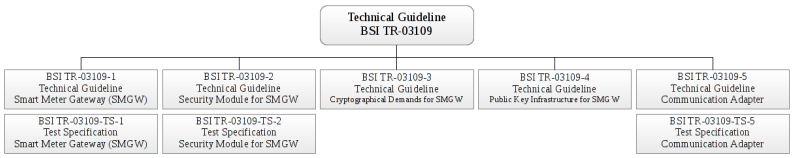
\includegraphics[width=1\textwidth]{images/BSI-TR-03109.png}
  \caption[Short description]{An example of a NILM analysis.}
  \label{fig:Appliance_Model}
\end{figure}
\todo{write design}

\cleardoublepage

%%% Local Variables:
%%% TeX-master: "diplom"
%%% End:
